\documentclass{article}
\usepackage[margin=1in,left=1.5in,includefoot]{geometry}
\usepackage{cite}
\newenvironment{problems}{\begin{list}{}{\setlength{\labelwidth}{.7in}}}{\end{list}} 
\usepackage{amsthm,amsfonts,amssymb,amsmath,graphicx} 
\graphicspath{./images/}
\usepackage[english]{babel}
\newtheorem{theorem}{Theorem}
\newtheorem{corollary}{Corollary}[theorem]
\newtheorem{lemma}{Lemma}
\newtheorem{definition}{Definition}
\usepackage{graphicx}
%\usepackage{textcomp}
\usepackage{xcolor}
\usepackage{amsmath}
\usepackage[english]{algorithm2e}
%\usepackage{setspace}
\usepackage{subfig} 
%\usepackage{array}
%%\usepackage{stfloats}
\usepackage{float} 
\usepackage{graphicx}
\usepackage{amsmath}
\usepackage{cite}
\usepackage{stackengine}
\usepackage{amsfonts,amsmath,amssymb}
\usepackage{multicol}
\usepackage{amsthm,amsfonts,amssymb,amsmath,graphicx}
\DeclareMathOperator*{\maxi}{maximize}
\begin{document}
	
	\begin{titlepage}
		\begin{center}
			\vspace*{1cm}
			
			\textbf{ \huge{ Report on\\\vspace{10pt} A Rate-Splitting Approach to the Gaussian Multiple-Access Channel}}
			\vspace{1.5cm}
			
			\textbf{Ritesh Kumar} \\
			\textbf{(EE20RESCH11005)}\\			
			\vspace{0.5cm}
			\textbf{Under the supervision of }\\
			\vspace{0.5cm}
			\textbf{Dr.Shashank Vatedka}\\
			\textbf{Assistant Professor}\\
			\textbf{ Department of Electrical Engineering}\\
			\textbf{IIT Hyderabad }
			\vfill			
		\end{center}
	\end{titlepage}
%	\tableofcontents
	\cleardoublepage
	\section{Introduction}
The main idea described in this paper is to put some light on the structure of the capacity region of the Gaussian multiple-access channel (MAC) and suggest a new and promising strategy for the implementation of a practical system.\par In this paper\cite{2}, the authors proposed a new scheme called rate splitting multiple-accessing (RSMA). This scheme allows user to split their data and signal into two parts. In this paper, authors  have considered,
\begin{itemize}
	\item Channel is discrete-time and frame synchronous with power constraint $P = (P_1, P_2, \dots )$ , where $P_i$ is power constraint for the user $i$ and noise variance $\sigma^2$
	\item Its capacity region is the subset of $\mathbf{R}^M$ containing rate tuples $(R_1,\dots R_M)$.
	\item Rate tuples component satisfying the condition
		\begin{equation}
			\sum_{i \in S}  R_i\leq \frac{1}{2}\log_2\left(1 + \frac{\sum_{i \in S} P_{i} }{\sigma^2} \right) \hspace{2mm} \forall S \subseteq \{ 1, \dots ,M\}
			\end{equation}
	 \begin{center}
		\begin{figure*}[htb!]
			\centering
			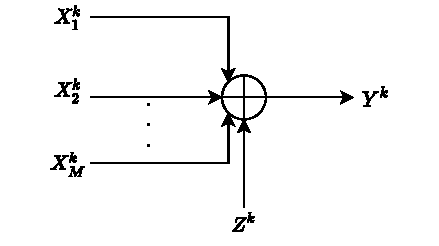
\includegraphics[height=.20\textheight]{pic1.pdf}
			\caption{Gaussian multiple-access channel}
			\label{fig1}
		\end{figure*}
	\end{center}
\item Where $Y^{k} = \sum_{i =1}^{M} X_{i}^{k} + Z^{k}$
	\end{itemize}
RSMA is a code-division multiple access scheme, for the M-user Gaussian multiple-access channel, for which the effort of finding the codes for M users of encoding and decoding is that of at most 2M-1 independent point-to-point Gaussian channels.
\begin{itemize}
	\item In this scheme decoder of user M can decode the data by considering the codewords of other users as Gaussian noise. Hence, the decoder of user M can decode considering the codewords of user $1, \dots M-1$ as noise. This kind of decoding procedure is known variously as onion peeling, stripping, and successive cancellation.
\end{itemize}
 \begin{center}
	\begin{figure*}[htb!]
		\centering
		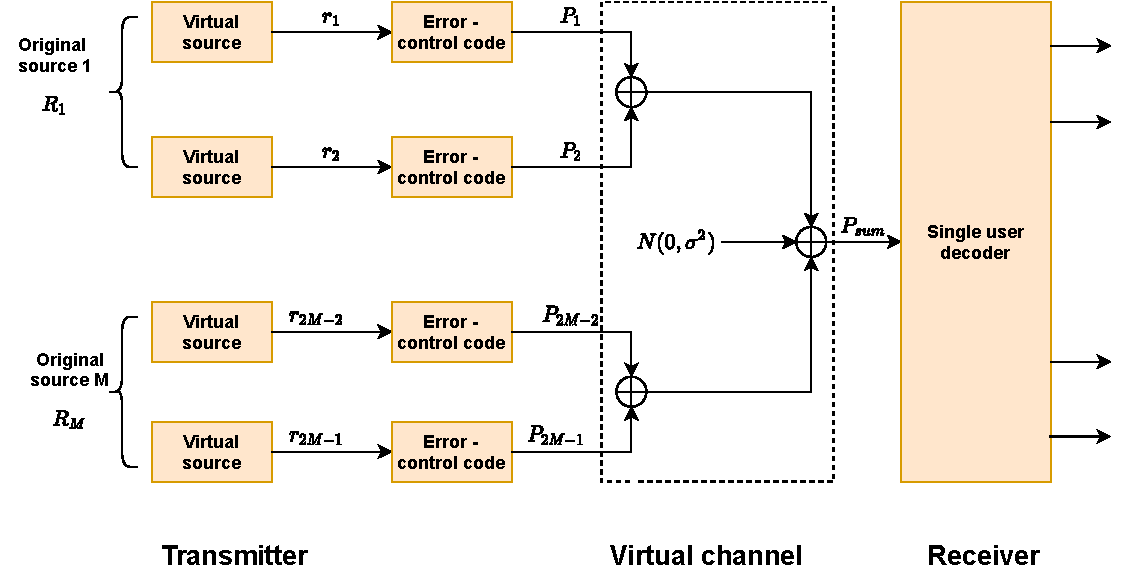
\includegraphics[height=.35\textheight]{pic_2.pdf}		
		\caption{A multiple-access system based on rate-splitting multiple accessing}
		\label{fig2}
	\end{figure*}
\end{center}
\newpage
\section{Vertex achievability by single user coding}

\begin{itemize}
	\item Vertices (corner) of the capacity region are indeed achievable via single user coding.
\item In figure \ref{fig3}(a) we do single-user decoding  for a two-user multiple-access system

\begin{center}
	\begin{figure*}[htb!]
		\centering
		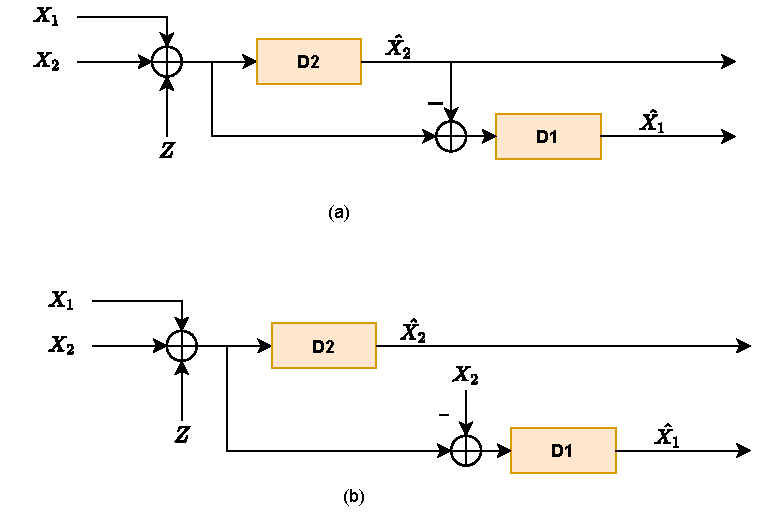
\includegraphics[height=.35\textheight]{pic_3.pdf}		
		\caption{(a) Single-user decoder (b) Genie-aided decoder}
		\label{fig3}
	\end{figure*}
\end{center}
 In figure \ref{fig3}(b) we consider the case where $X_2$ is always removed from the input to $D1$. The rest of the procedure is the same in both. In first part of the figure \ref{fig3} we  decode $X_2$ first then we decode $X_1$ $X_1$ by subtracting estimated value of $X_2$ from the received codeword. But in the second case which is ''Genie-aided decoder'', which follows the Wozencraft and Jacobs Postulate\cite{1}, $D_1$ always knows the value of $X_2$ and then decode the value of  $X_1$.
\end{itemize}
\section{Rate-splitting multiple accessing achieves any point in the capacity region}
Consider $C(P, \sigma^2)$ as the capacity of  a white Gaussian noise channel with power $P$ and  noise $\sigma^2$, hence,
\begin{equation}
	C = \frac{1}{2}\log_2\left( 1 + \frac{P}{\sigma^2}\right)
\end{equation}
With the help of chain rule we can verify that,
\begin{equation}
	C(P, \sigma^2) = C(P_1, \sigma^2) + C(P_2, \sigma^2 + P_1) \label{3}
\end{equation}
equation \eqref{3} is valid for all nonnegative number $P_1, P_2,$ and $\sigma^2$ such that $P = P_1 + P_2$. The chain rule says that the rate R of a single user transmitting at capacity can be seen as vertex 
\begin{equation}
	\left( R_1, R_2 \right) = \left( C(P_1, \sigma^2), C(P_2, \sigma^2+P_1)\right) \label{4}
\end{equation} \cite{3}
equation \eqref{4} shows the vertex point of a two user virtual channel described by $\left(P-1, P
_2\right)$ and $\sigma^2$, where $P_1 + P_2 = P\text{and}, R_1 +R_2 = R$.\paragraph{ The advantage of splitting the user of the point-to-point channel into two virtual users may be seen as, we can achieve a higher rate code from the two lower rate codes.}
\flushleft Let consider a two user case for the more illustrative of the idea behind rate splitting.Let the noise variance is $\sigma^2$ and power constraint $\left( P_1 ,P_2\right)$ be arbitrary, and consider any rate tuple $(R_1, R_2)$ in the dominant face of capacity region\cite{4} such that,
\begin{align*}
	R_1< C(P_1, \sigma^2)\\
	R_2 < C(P_2, \sigma^2) \\
	R_1+ R_2 = C(P_1 +P_2 , \sigma^2)
\end{align*}
\begin{center}

	\begin{figure}[htb!]
		\centering
		\includegraphics[height=.3 \textheight]{fig_11.png}
		\caption{Dominant face of capacity region}
		\label{fig11}
	\end{figure}
\end{center}
 Let $\delta>0$ be the unique number wich satisfies,
\begin{equation}
	R_2 = C(P_2, \sigma^2 + \delta)
\end{equation}
Now consider Gaussian MAC with noise power $\sigma^2$ and there is 3 virtual inputs. Power constraint is $(p_1,p_2,p_3)$ such that, 
\begin{align*}
	p_1 = \delta\\ p_2 = P_2 \\ p_3 = P_1 -\delta
\end{align*}
Rate tuple $\left( r_1, r_2, r_3\right)$ is ,
\begin{align*}
	r_1 = C(p_1,  \sigma^2)\\ r_2 = C (p_2, \sigma^2 +p_1) \\r_3 =C (p_2, \sigma^2 +p_1+p_2)
\end{align*}
Virtual user 2 has the same rate and power constraint as the original user 2. We can also observe that,
\begin{align*}
	r_1 +r_2 +r_3 = C(p_1+p_2 +p_3,  \sigma^2)\\  = C (P_1 +P_2, \sigma^2 ) = R_1 +R_2
\end{align*}
Hence we can observe here user does need not to know at what rate user two is operating as long as his rate is known since there is no constraint on the rate of user one w.r.t user 2. And this helps a particular user to operate in the dominant face of the capacity region (more precisely on the capacity boundary without considering the operating region of another user). \newline 

The geometrical relationship between $R = (R_1, R_2)$ and $r = (r1,r2,r3)$ is that, they will lie on dominant face of capacity region. Define the quardruple $\left( M, P, R, \sigma^2\right)$ and a nonnegative $\delta_i$, $i = 1, \dots , M$ that satisfies
\begin{equation}
	R_i = C(P_i, \delta_i+\sigma^2)
\end{equation}
\begin{figure}[htb!]
\begin{center}
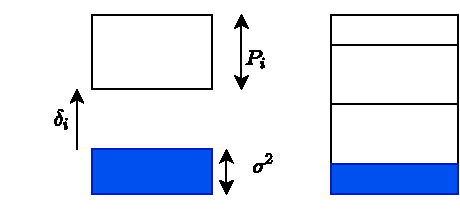
\includegraphics[height=.2\textheight]{pic_6.pdf}
\caption{Block representation}
\label{fig6}
\end{center}
\end{figure}
The bottom box (in blue) in figure \ref{fig6} represent the noise and, its height is propositional to the noise and power $\sigma^2$. The user is represented by the white rectangle whose height is proportional to power constraint $P$ and to $\delta$ respectively. Width represents nothing. it's just for convenience. \newline
For generalization for M-user author proposed two lemmas as, lemma 1 and lemma 2.


\begin{lemma}
For a tight configuration $\left( M, P, R, \sigma^2\right)$ after a possible re-indexing, there exists at least one index $i$ for which 
	\begin{equation}
		\delta_i \leq \delta_{i+1}\leq \delta_i + P_i \label{7}
	\end{equation}
\end{lemma}
Here, tight configuration means  $\delta_i$ is very small.
\begin{proof}
	We re-index so that $ 0=\delta_0 \leq \delta_1 \leq \delta_2 \dots , \leq \delta_M $ and assume that assume that claim is false i.e., that
	\begin{equation}
		\delta_{i+1} > \delta_i + P_i, i = 0,1, \dots, (M-1)
	\end{equation}
	It follows that
	
	
	\begin{equation}
		\sum_{i =1}^{M} R_i = \sum_{i=1}^{M} C(P_i, \sigma^2+\delta_i)<  \sum_{i=1}^{M} C \left( P_i, \sigma^2+\delta_i  + \sum_{j<j} P_i \right) = C \left(  \sum_{i=1}^{M} P_i, \sigma^2 \right) \label{9}
	\end{equation}
This is not possible since according to the assumption we have to consider optimal rate i.e we are operating on the boundary of the capacity region. So inequality given in \eqref{9} is not possible. Hence there must exist a $\delta_i$ that satisfies \eqref{7}.
	\begin{lemma}
		Consider a quadruple $\left( M,P,R \sigma^2 \right)$ and asumme that
		\begin{equation}
			\delta_j \geq \delta_i +P_i \label{8}
		\end{equation}
		for some $i,j \in \left\{ 1,2, \dots, M\right\}$. Let $\delta$ be the unique nonnegative number such that $R_i +R_j = C \left( P_i + P_j , \delta \right).$ Then
		\begin{equation}
			\delta_i \leq \delta \leq \delta_j - P_i \label{9}
		\end{equation}
		That is if two ''nonoverlapping'' users are combined by putting their power together, to keep their sum-rate constant, the bottom user has to move down.
		\begin{proof}
			The  inequaltiy  \eqref{9} follows from the raltion from,
			\begin{align}
				C\left(P_i+P_j, \delta \right) = R_i + R_j = C \left(P_i, \delta_i \right) + C \left(P_j, \delta_j \right) \\ \leq  C \left(P_i, \delta_i \right) + C \left(P_j, \delta_j + P_i \right)  \\  =  C \left(P_i +P_j, \delta_i \right) 
			\end{align}
			srict inequaltiy given in \eqref{8} follows from,
			\begin{align}
				C\left(P_i+P_j, \delta \right) = R_i + R_j = C \left(P_i, \delta_i \right) + C \left(P_j, \delta_j \right)  \\ \geq  C \left(P_i, \delta_i -p_i \right) + C \left(P_j, \delta_j  \right) \\ =  C \left(P_i +P_j, \delta_i-P_i \right) 
			\end{align}
		\end{proof}
	\end{lemma}
	The notion of the splitting users into virtual users and channel inputs  in a meaniningful ways is formalized by the following definition.
	\begin{definition}
		The quadruple $\left(m,p,r, \sigma^2 \right)$ is a spinoff of $\left(M, P R, \sigma^2 \right)$ if there exist a surjective mapping $\phi : \left\{ 1, \dots , m\right\} \rightarrow \left\{ 1, \dots, M\right\}$ such that for all $ i \in \left\{ 1, \dots, M \right\}$ we have 
		\begin{equation}
			P_i \geq \sum_{j \in \phi^{-1}(i)} p_j
		\end{equation} 
		\text{and}
\begin{equation}
	R_i \leq \sum_{j \in \phi^{-1} }r_j
\end{equation}
where $\phi^{-1}(i)$ is the set of all $j \in \left\{ 1, \dots, m\right\}$ that map into $i$ by mean of $\phi$
	\end{definition}
\begin{theorem}
	For every M-user configuration $\left(M, P, R, \sigma^2 \right)$ there exist a spinoff $\left( m,p,r, \sigma^2\right)$ which is single-user-codable.Moreover, one can guarantee that one user is un-split and that no user split into more thantwo virtual users. Hence $m\leq 2M-1$
\end{theorem}

Proof :\\
Without loss of generality we may assume that $\left(M,P,R,\sigma^2\right)$ is tight. By induction on M, we can prove this. for M = 1 the claim is trivially true. Consider 2 user cases, i.e. M=2. Any rate tuple $(R_1, R_2)$ in the dominant face of the capacity region such that,
	\begin{align*}
		R_1< C(P_1, \sigma^2)\\
		R_2 < C(P_2, \sigma^2) \\
		R_1+ R_2 = C(P_1 +P_2 , \sigma^2)
	\end{align*}
	let $\delta >0 $ be a unique number such that,
	\begin{equation}
		R_2 = C(P_2 , \sigma^2 + \delta)
	\end{equation}
Now we assume that, it is true for an arbitrary positive M and consider the case of M+1 users. Using lemma 1 we may assume that,
$\delta_M \leq \delta_{M+1}$ and $\delta_{M+1}\leq \delta_M +P_M$, We reduce the original (M+1) user configuration $\left(M+1, P,R, \sigma^2\right)$ to an M-user configuration $\left(M,\hat{P}, \hat{R}, \sigma^2\right)$ where,\\
\begin{align*}	
	\hat{P_i} = P_i, i = 1,2, \dots, M-1\\
	\hat{P_M} = P_M + P_{M+1},\\   \hat{R_i} = R_i,   i = 1,2, \dots, M-1 \\  \hat{R_M} = R_M + R_{M+1}
\end{align*}
By the induction hypothesis, there exist a spinoff $\left(m,p, r, \sigma^2 \right)$ of $\left(M, P, R,\sigma^2 \right)$ with m $\leq$2M-1 and with the property that one user is unsplit and no user is split into more than two users.

\begin{figure}[htb!]
	\centering
	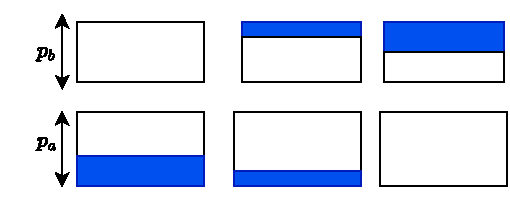
\includegraphics[height=.20\textheight]{pic_8.pdf}
	\caption{Block representation}
	\label{fig7}
\end{figure}
The author claimed that for better decoding and encoding procedure, we have to perform splitting, at most into two virtual users and at least one user must be unsplitted. That is for low complex coding and irrespective of the information of another user particularly power constraints. If we split the user into more than two virtual sources, then we are not able to achieve the optimal rate in the capacity region. This is represented in figure \ref{fig7}. Where $\hat{P_i} = p_a + p_b $ and corresponding rate is  $\hat{R_i}$
\begin{figure}[htb!]
	\centering
	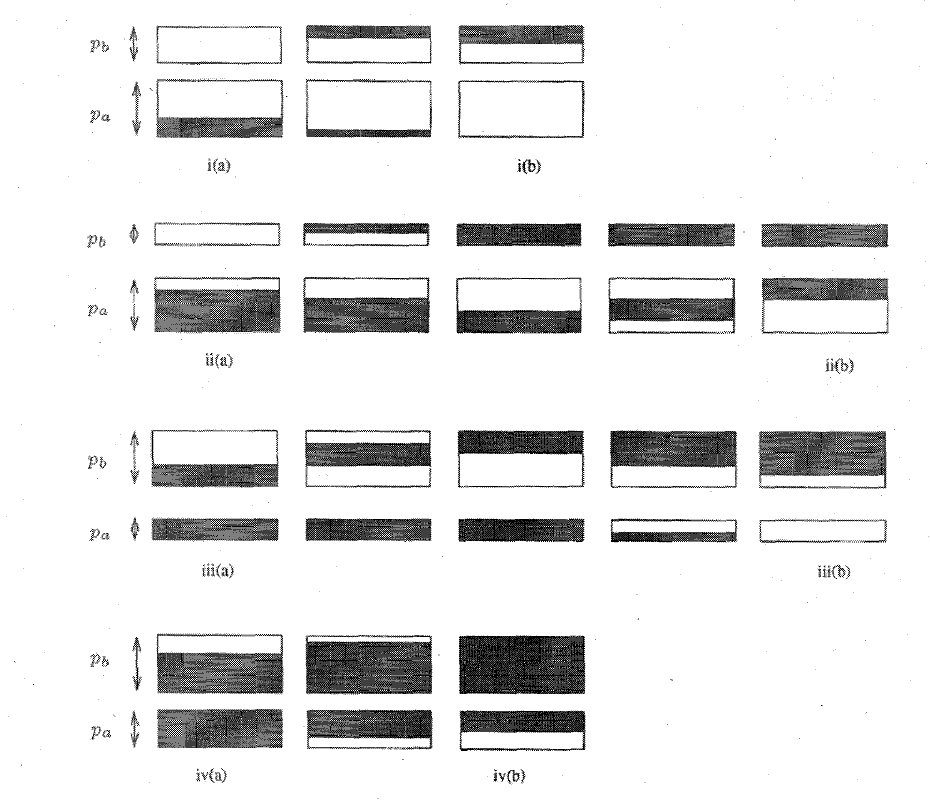
\includegraphics[height=.3\textheight]{fig_9.png}
	\caption{Block representation}
	\label{fig8}
\end{figure}
\end{proof}
 \section{Advantages of RSMA}
Any point in the capacity region of a discrete-time synchronous Gaussian MAC is achievable via RSMA at relatively low coding complexity. There is no need for synchronization among users. Spread-spectrum multiple access (SSMA) has an upper bound on the spectral efficiency as, there is no such upper bound for RSMA. For discrete-time Gaussian MAC, one can achieve rate tuples via the "time-sharing" approach. For continuous-time channel one can also do "frequency-sharing between vertices"
Interference reduction resulting from intermittent transmitters. Cellular reuse factor of 1 for RSMA.
Channel estimation is better than a narrowband system. There is no near-far problem in RSMA like SSMA. RSMA allows one to achieve any point in the capacity region of a time-varying multipath channel. It allows the user to use his extra power for the benefit of another user. That is if user 1 is willing to increase his power to the point that he can achieve his rate viewing the user as noise, then user 2 can transmit the same rate as if the channel were entirely dedicated to him..


\section{Further research}
 How RSMA behaves with the practical codes is not addressed by the author. What is the effect of the imperfect cancellation at the receiver is also an area to discover and need further research. Effect on the Rate with various coding schemes like turbo coding is further research needed to find an entire family of such codes with rates that vary over a broad range.
\bibliographystyle{ieeetr}
\bibliography{citation}


\end{document}